\chapter{Fasediagram (portræt?)}
Fasediagrammer er anvendelige i forhold til at illustrere differentialligningssystemer og dermed skabe overblik over opførslen omkring ligevægtspunkter i systemet.

Dette afsnit er baseret på \citep[s. 488-490]{EP}. \\
Der er givet et system af differentialligninger:

\begin{equation}
    \begin{aligned}
    &\frac{dx}{dt}=F(x,y),\\ 
    &\frac{dy}{dt}=G(x,y)
    \end{aligned}
\end{equation}

Vi kan danne os et overblik over løsningerne til det givne system ved at konstruere et billede, der viser systemets ligevægtpunkter sammen med løsningskurver i $xy$-planet. Dette kaldes et faseportræt, da det illustrere systemets ændringer over tid. \\
\hfill \break
Hvis man ikke med det samme kan gennemskue løsningen til en ODE eller et system, så for at få en idé om hvordan løsningerne kunne se ud kan man konstruere et linjeelement i et $xy$-plan. Her tegner man linjestykker med hældingen:    
$$\frac{dy}{dx}=\frac{y'}{x'}=\frac{G(x,y)}{F(x,y)}$$

\begin{Example}
\hfill \break
\textnormal{Betragt differentialligning systemet:} 

\begin{equation}\label{DLS}
    \begin{aligned}
    &F(x,y)= x'=x-y\\ 
    &G(x,y)=y'=1-x^2
    \end{aligned}
\end{equation}

\textnormal{Med ligevægtspunkterne:} $$(-1,-1) \ \textnormal{og} \ (1,1)$$
\textnormal{}

\textnormal{Ved at kigge på et par tilfældige punkter i $xy$-planet, indsætter deres værdi i (\ref{DLS}) og dermed finde ud af hvad punktets hældning er.} 

\begin{center}
  \begin{tabular}{ | c || c | c | c | c | c |}
    \hline
    x & 0 & 1 & -1 & 0 & $\hdots$ \\ \hline 
    y & 1 & 1 & -1 & -1 & $\hdots$\\ \hline
    $\frac{G(x,y)}{F(x,y)}$ & -1 & 0 & 0 & 1 & $\hdots$\\ \hline
  \end{tabular}
\end{center}

\textnormal{Udfra disse punkter, kan man tegne et linjestykke i hver af punkterne med deres hældning.}

\begin{center}
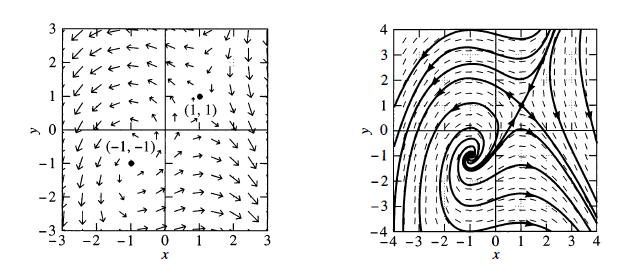
\includegraphics[width=15cm, height=6cm]{slope}
\end{center}
\captionof{figure}{Et linjeelement og et faseportæt til differentialligning systemet $F(x,y)$ og $G(x,y)$}\label{slope}
\hfill \break

\textnormal{På Figur \ref{slope} kan man se hvordan løsningskurverne til i faseportrættet følger linjestykkerne i linjeelementet, og dermed også bevæger sig hhv. hen  imod eller væk fra ligevægtpunkterne.}

\end{Example}

